% =====================================================================
% Q1 Schema Graph (Assignment 2)
%   - 8 tables  -> 8 nodes
%   - each foreign key -> 1 edge, drawn FK -> referenced PK (20 edges)
%   - each table lists only its PK and FK columns
%   Source of tables and keys: SCHEMA.md of the course repo
%   Compile: pdflatex schema_graph_q1.tex
% =====================================================================
\documentclass[tikz,border=10pt]{standalone}
\usetikzlibrary{shapes.multipart, arrows.meta}
\renewcommand{\familydefault}{\sfdefault}

% ---------- key labels ----------
\definecolor{keyblue}{HTML}{3B5BDB}   % colour of PK / FK labels
\definecolor{headbg}{HTML}{DCE8F5}    % header fill
\definecolor{edge}{HTML}{2F3E9E}      % line colour
\newcommand{\PK}{(\textcolor{keyblue}{\textbf{PK}})}
\newcommand{\FK}{(\textcolor{keyblue}{\textbf{FK}})}

% ---------- styles ----------
\tikzset{
  % A table is ONE box split into rows (TikZ "rectangle split").
  % Row names used for anchors:
  %   text  = row 1 = table name (shaded)
  %   two   = row 2 = primary key
  %   three, four, five, ... = foreign keys
  % Anchor example: (Issues.four east) = right edge of row 4 of Issues.
  table/.style={
    rectangle split, rectangle split parts=#1, draw, anchor=north west,
    rectangle split draw splits=false,             % no line under every row
    rectangle split part fill={headbg, white},   % header shaded, rows white
    inner ysep=4pt,
    text width=4.4cm, align=left, font=\small
  },
  % FK edge: dot at the FK row, arrow at the referenced PK row.
  fk/.style={{Circle[length=1.8mm]}-{Latex[length=2.8mm]}, line width=1.4pt, edge},
  % Small dot where an edge turns into a vertical channel (shows where edges join).
  junction/.style={circle, fill=edge, inner sep=1.4pt},
}

\begin{document}
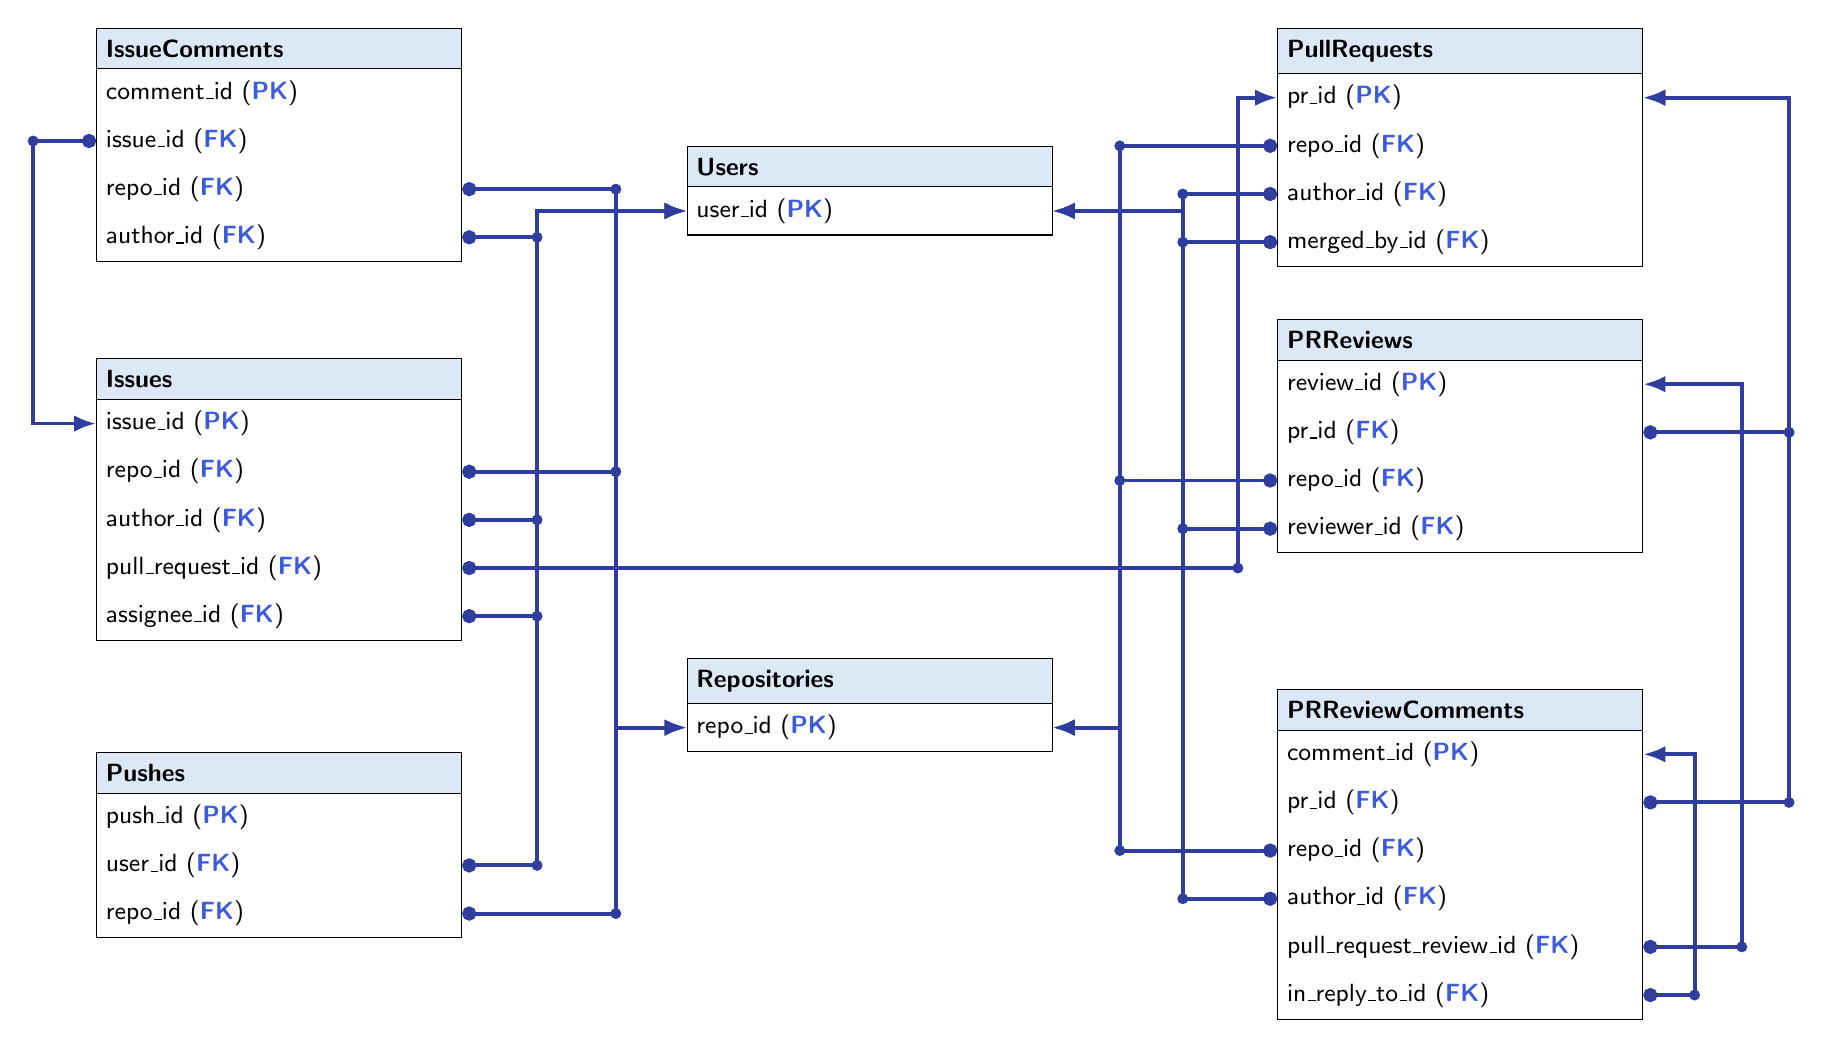
\begin{tikzpicture}

% =====================================================================
% 1) NODES: the 8 tables
%    left column  : IssueComments, Issues, Pushes
%    middle column: Users, Repositories (referenced by most tables)
%    right column : PullRequests, PRReviews, PRReviewComments
% =====================================================================

% ---------------- middle column ----------------
\node[table=2] (Users) at (7.5, -1.5) {
  \textbf{Users}
  \nodepart{two}   user\_id \PK
};

\node[table=2] (Repos) at (7.5, -8) {
  \textbf{Repositories}
  \nodepart{two}   repo\_id \PK
};

% ---------------- left column ----------------
\node[table=5] (IssueComments) at (0, 0) {
  \textbf{IssueComments}
  \nodepart{two}   comment\_id \PK
  \nodepart{three} issue\_id \FK
  \nodepart{four}  repo\_id \FK
  \nodepart{five}  author\_id \FK
};

\node[table=6] (Issues) at (0, -4.2) {
  \textbf{Issues}
  \nodepart{two}   issue\_id \PK
  \nodepart{three} repo\_id \FK
  \nodepart{four}  author\_id \FK
  \nodepart{five}  pull\_request\_id \FK
  \nodepart{six}   assignee\_id \FK
};

\node[table=4] (Pushes) at (0, -9.2) {
  \textbf{Pushes}
  \nodepart{two}   push\_id \PK
  \nodepart{three} user\_id \FK
  \nodepart{four}  repo\_id \FK
};

% ---------------- right column ----------------
\node[table=5] (PullRequests) at (15, 0) {
  \textbf{PullRequests}
  \nodepart{two}   pr\_id \PK
  \nodepart{three} repo\_id \FK
  \nodepart{four}  author\_id \FK
  \nodepart{five}  merged\_by\_id \FK
};

\node[table=5] (PRReviews) at (15, -3.7) {
  \textbf{PRReviews}
  \nodepart{two}   review\_id \PK
  \nodepart{three} pr\_id \FK
  \nodepart{four}  repo\_id \FK
  \nodepart{five}  reviewer\_id \FK
};

\node[table=7] (PRReviewComments) at (15, -8.4) {
  \textbf{PRReviewComments}
  \nodepart{two}   comment\_id \PK
  \nodepart{three} pr\_id \FK
  \nodepart{four}  repo\_id \FK
  \nodepart{five}  author\_id \FK
  \nodepart{six}   pull\_request\_review\_id \FK
  \nodepart{seven} in\_reply\_to\_id \FK
};

% ---- one line under each header (the only divider inside a table) ----
% "text split" = the border between row 1 (header) and row 2.
\foreach \t in {Users, Repos, IssueComments, Issues, Pushes,
                PullRequests, PRReviews, PRReviewComments}
  \draw (\t.text split west) -- (\t.text split east);

% =====================================================================
% 2) EDGES: the 20 foreign keys, grouped by the referenced table
%
%    Every edge is a right-angle line through a vertical "channel":
%      \draw[fk] (FK row) -- (FK row -| channel) node[junction]{} |- (PK row);
%      (A -| ch) = the point with A's height and ch's x position
%      |-        = go vertical first, then horizontal into the PK row
%    Edges to the same PK share one channel, so they join into one line.
% =====================================================================

% ---- channels (vertical lanes, only their x position matters) ----
\coordinate (chUsersL)  at (5.6, 0);   % left tables  -> Users
\coordinate (chReposL)  at (6.6, 0);   % left tables  -> Repositories
\coordinate (chReposR)  at (13.0, 0);  % right tables -> Repositories
\coordinate (chUsersR)  at (13.8, 0);  % right tables -> Users
\coordinate (chPRfromI) at (14.5, 0);  % Issues -> PullRequests
\coordinate (chIssues)  at (-0.8, 0);  % IssueComments -> Issues (left side)
\coordinate (chSelf)    at (20.3, 0);  % PRReviewComments -> itself
\coordinate (chReviews) at (20.9, 0);  % PRReviewComments -> PRReviews
\coordinate (chPR)      at (21.5, 0);  % PRReviews / PRReviewComments -> PullRequests

% ---- -> Users.user_id (8 edges) ----
\draw[fk] (IssueComments.five east)    -- (IssueComments.five east -| chUsersL)    node[junction]{} |- (Users.two west); % IssueComments.author_id
\draw[fk] (Issues.four east)           -- (Issues.four east -| chUsersL)           node[junction]{} |- (Users.two west); % Issues.author_id
\draw[fk] (Issues.six east)            -- (Issues.six east -| chUsersL)            node[junction]{} |- (Users.two west); % Issues.assignee_id
\draw[fk] (Pushes.three east)          -- (Pushes.three east -| chUsersL)          node[junction]{} |- (Users.two west); % Pushes.user_id
\draw[fk] (PullRequests.four west)     -- (PullRequests.four west -| chUsersR)     node[junction]{} |- (Users.two east); % PullRequests.author_id
\draw[fk] (PullRequests.five west)     -- (PullRequests.five west -| chUsersR)     node[junction]{} |- (Users.two east); % PullRequests.merged_by_id
\draw[fk] (PRReviews.five west)        -- (PRReviews.five west -| chUsersR)        node[junction]{} |- (Users.two east); % PRReviews.reviewer_id
\draw[fk] (PRReviewComments.five west) -- (PRReviewComments.five west -| chUsersR) node[junction]{} |- (Users.two east); % PRReviewComments.author_id

% ---- -> Repositories.repo_id (6 edges) ----
\draw[fk] (IssueComments.four east)    -- (IssueComments.four east -| chReposL)    node[junction]{} |- (Repos.two west); % IssueComments.repo_id
\draw[fk] (Issues.three east)          -- (Issues.three east -| chReposL)          node[junction]{} |- (Repos.two west); % Issues.repo_id
\draw[fk] (Pushes.four east)           -- (Pushes.four east -| chReposL)           node[junction]{} |- (Repos.two west); % Pushes.repo_id
\draw[fk] (PullRequests.three west)    -- (PullRequests.three west -| chReposR)    node[junction]{} |- (Repos.two east); % PullRequests.repo_id
\draw[fk] (PRReviews.four west)        -- (PRReviews.four west -| chReposR)        node[junction]{} |- (Repos.two east); % PRReviews.repo_id
\draw[fk] (PRReviewComments.four west) -- (PRReviewComments.four west -| chReposR) node[junction]{} |- (Repos.two east); % PRReviewComments.repo_id

% ---- -> PullRequests.pr_id (3 edges) ----
\draw[fk] (Issues.five east)            -- (Issues.five east -| chPRfromI)       node[junction]{} |- (PullRequests.two west); % Issues.pull_request_id
\draw[fk] (PRReviews.three east)        -- (PRReviews.three east -| chPR)        node[junction]{} |- (PullRequests.two east); % PRReviews.pr_id
\draw[fk] (PRReviewComments.three east) -- (PRReviewComments.three east -| chPR) node[junction]{} |- (PullRequests.two east); % PRReviewComments.pr_id

% ---- -> Issues.issue_id (1 edge) ----
\draw[fk] (IssueComments.three west) -- (IssueComments.three west -| chIssues) node[junction]{} |- (Issues.two west); % IssueComments.issue_id

% ---- -> PRReviews.review_id (1 edge) ----
\draw[fk] (PRReviewComments.six east) -- (PRReviewComments.six east -| chReviews) node[junction]{} |- (PRReviews.two east); % PRReviewComments.pull_request_review_id

% ---- -> PRReviewComments.comment_id (1 edge, points to its own table) ----
\draw[fk] (PRReviewComments.seven east) -- (PRReviewComments.seven east -| chSelf) node[junction]{} |- (PRReviewComments.two east); % PRReviewComments.in_reply_to_id

\end{tikzpicture}
\end{document}
